\documentclass{article}%
\usepackage[T1]{fontenc}%
\usepackage[utf8]{inputenc}%
\usepackage{lmodern}%
\usepackage{textcomp}%
\usepackage{lastpage}%
\usepackage[head=40pt,margin=0.5in,bottom=0.6in]{geometry}%
\usepackage{graphicx}%
%
\title{\textbf{Madres heroínas. Humanismo}}%
\author{CARLOS SAINZ MUÑOZ}%
\date{04/03/2019}%
%
\begin{document}%
\normalsize%
\maketitle%
\textbf{URL: }%
http://www.eluniversal.com/el{-}universal/34528/madres{-}heroinas{-}humanismo\newline%
%
\textbf{Periodico: }%
EU, %
ID: %
34528, %
Seccion: %
el{-}universal\newline%
%
\textbf{Palabras Claves: }%
NO\_TIENE\newline%
%
\textbf{Derecho: }%
2.1%
, Otros Derechos: %
\newline%
%
\textbf{\textit{La UE, la ONU y OEA han manifestado su apoyo para mediar el ingreso y distribución con la Cruz Roja, esto sería un acto de humanismo generoso al pueblo valiente para que se salga de la crisis}}%
\newline%
\newline%
%
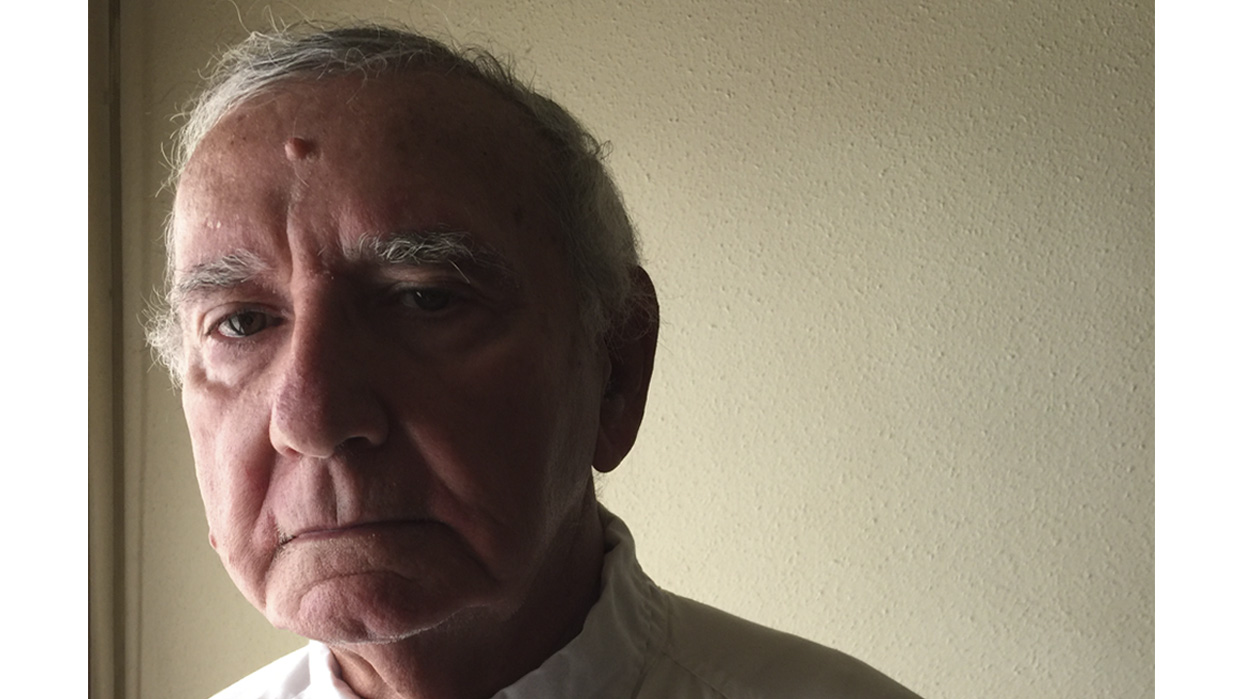
\includegraphics[width=300px]{EU_34528.jpg}%
\newline%
%
Especial significación, respeto y solidaridad activa, merecen esas mujeres excepcionales como son las madres trabajadoras, bien sean las obreras, profesionales,  y las amas de casa que  enfrentan una crisis permanente que   ha generado la necesidad de una ayuda humanitaria inminente y urgente ante la grave  crisis que afecta los DDHH del pueblo. Ellas han  tenido   con valentía ante las situaciones agravantes y difíciles, con salarios  con  hiperinflación insuficientes, con dificultad  y carestías de productos básicos, alimenticios, medicinas y la de asumir las migraciones producto  de las   circunstancias adversas para mantener sus familias, hijos, embarazos, enfermos y ancianos  que conforman el núcleo familiar. Situaciones  que son hechos públicos y notorios las han  asumido con responsabilidad, valentía y alto sentido  familiar,   como  verdaderas heroínas, por ello son ejemplo a seguir y admirar.%
\newline%
%
Las madres migrantes en adición a lo anterior   han tenido que asumir   el rol de emigrar a otros países  para tratar de enfrentar las graves condiciones de supervivencia y conseguir en otros países las condiciones mínimas para que sus hijos y demás familiares  obtengan  lo que aquí se les imposibilita para sobrevivir.%
\newline%
%
Si hay un colectivo social del trabajo de profunda   trascendencia y humanismo  universal que a través de distintas épocas es difícil y mezquino de ignorar  a las madres trabajadoras es la lucha infatigable e inconclusa  por los derechos humanos universales  en el espacio y en el tiempo. (La ONU instituyó  un día internacional de las madres ).%
\newline%
%
La lucha emprendida por las madres por la ayuda alimentaria  y ante  la situación  tan  grave  que vivimos, ha sido  y  es dura y es lamentable  que no se lograra su paso ya que la gran  mayoría de los países latinoamericanos  y europeos  la dieron para auxiliar al pueblo y a legiones de migrantes. Es justo reconocerlas como  heroínas valientes anónimas que  nunca podremos olvidar, Dios las  bendiga.%
\newline%
%
La UE, la ONU y OEA han manifestado su apoyo para mediar el  ingreso y distribución con la Cruz Roja, esto  sería  un acto de humanismo   generoso al  pueblo Valiente  para que se salga de una crisis humanitaria inmerecida.%
\newline%
%
@laborasainz%
\newline%
%
\end{document}